   
\chapter{Literature Review} 

% \todo[inline]{Todo capítulo deve ter uma introdução explanatória. "This chapter describes"}

    This chapter provides a comprehensive literature review of the key technologies and concepts that form the foundation of this dissertation. It begins with an overview of the applications of Artificial Intelligence (AI) in the Exploration and Production (E\&P) industry. The focus then narrows to Large Language Models (LLMs), discussing their architecture and impact. Subsequently, the chapter delves into the Retrieval-Augmented Generation (RAG) technique, which enhances LLMs with external knowledge. It also explores the use of single and multi-agent setups. Finally, the chapter concludes by examining the 'LLM-as-judge' paradigm for evaluating the performance of generative models.


    \section{AI in the Exploration and Production (E\&P) industry}

        The use of AI in the Exploration and Production (E\&P) industry has been extensive. 
        In the last decades the majority of AI applications in the industry involved data mining and neural networks \citep{Bravo2014}. 
        An example is the work by \citep{Gudala2021} on optimization of the properties of the heavy oil flow, through the use of neural networks to optimize flow-influencing parameters.
        Another development was a deep learning workflow proposed by \citep{Gohari2024}, with the generation of synthetic graphic well logs through the application of transfer learning. 
        These developments illustrate the potential of AI to improve processes and the accuracy and efficiency of data analysis \citep{Rahmani2021}.
    
        Natural Language Processing (NLP) stands at the intersection of computer science and linguistics, representing a domain within artificial intelligence aimed at enabling computers to understand and process human language in a way that is both meaningful and effective \citep{Liddy2001}. 
        This field integrates a diverse range of computational techniques to analyze and represent text at various levels of linguistic detail, striving to emulate human-like language understanding. 
        As an active area of research, traditionally NLP employs multiple layers of language analysis, each contributing uniquely to the interpretation and generation of language, which finds practical applications in various sectors \citep{Liddy2001}.      
        In the O\&G industry, the management of unstructured data, such as texts, images, and documents, is crucial, with Natural Language Processing (NLP) and Machine Learning playing key roles.
        Research by \citet{Antoniak2016} and \citet{Castineira2018} has explored the use of NLP to analyze risks and drilling reports.           
    
    \section{Natural Language Processing}

        NLP (Natural Language Processing) is a broad field that covers various tasks to enable computers to process and understand human language. These tasks, which represent specific problems or applications, have been the focus of research for decades, predating the recent surge in Large Language Models. They range from fundamental challenges like part-of-speech tagging to complex applications like machine translation. This section explores two tasks particularly relevant to this dissertation: Question Answering (Q\&A) and Text-to-SQL, both of which have been significantly advanced by recent developments in the field.

        \subsection{Q\&A tasks}     

            Question and Answer (Q\&A) represent a method to facilitate knowledge transfer between individuals within organizations \citep{Iske2005}. 
            \xexeo{As tasks vem antes das LLMs, elas sempre existiram como problemas da área de NLP. Inclusive acho que na seção de NLP você pode fazer um parágrafo sobre a existência de várias tasks e usar essas como subseções}
            \vitor{Feito}
            Conceptually, Q\&A systems are designed to connect individuals who possess specific knowledge with those seeking that knowledge through a structured question-and-answer format. 
            The role of Q\&A in the documentation landscape, as exemplified by platforms such as Stack Overflow, highlights their significance in technical disciplines \citep{Treude2011}. 
            This understanding can guide organizations in making more informed decisions about implementing such systems to enhance knowledge transfer and organizational learning \citep{Iske2005}.

        \subsection{Text-to-SQL tasks} 

            Text-to-SQL tasks in the context of artificial intelligence involve the automatic translation of natural language questions or commands into structured SQL (Structured Query Language) queries \citep{Qin2022}. This is an important area in natural language processing (NLP), allowing users to interact with databases using plain language rather than needing to know how to write complex SQL queries.         
                
            The arrival of advanced language models like GPT-3 and GPT-4 \citep{OpenAImodels} has marked a significant leap in Text-to-SQL applications \citep{Singh2023}, demonstrating remarkable capabilities in handling these tasks. This can be attributed to their extensive training on diverse datasets \citep{Deng2021}, which include not only large amounts of text but also structured data like tables and code, enabling the model to understand the intricate relationships between language and data structures. The study by \citep{Deng2023} introduces a pre-training framework for text to SQL translation, emphasizing the alignment between text and tables in Text-to-SQL tasks.





    \section{Large Language Models}         

        Large Language Models (LLMs) are advanced neural network-based models designed to understand and generate human-like text. 
        They leverage the Transformer architecture introduced in the seminal paper \enquote{Attention is All You Need} by \citet{Vaswani2017}. 
        This architecture relies on self-attention mechanisms, allowing the model to weigh the importance of different words in a sentence effectively. 

        The emergence of LLMs has made it possible to understand and produce textual information. 
        These systems are expected to revolutionize various industries by supporting complex decision-making processes. GPT models \citep{OpenAI2023}, in particular, take advantage of its vast training data to provide human-like responses \citep{Mosser2024}, which can be highly beneficial in contexts requiring natural language understanding and generation. The exponential growth in the size and capability of LLMs in recent years has been remarkable. Models like OpenAI's GPT series have shown significant advancements, moving from millions to hundreds of billions of parameters, which gives them increasingly sophisticated natural language understanding and generation. This advancement is illustrated in Figure~\ref{fig:llm_evolution}.

        \xexeo{Acho que aqui merecia um gráfico do crescimento do tamanho das LLMs e um parágrafo sobre esse crescimento}
        \vitor{Feito}

        \begin{figure}[ht]
            \centering
            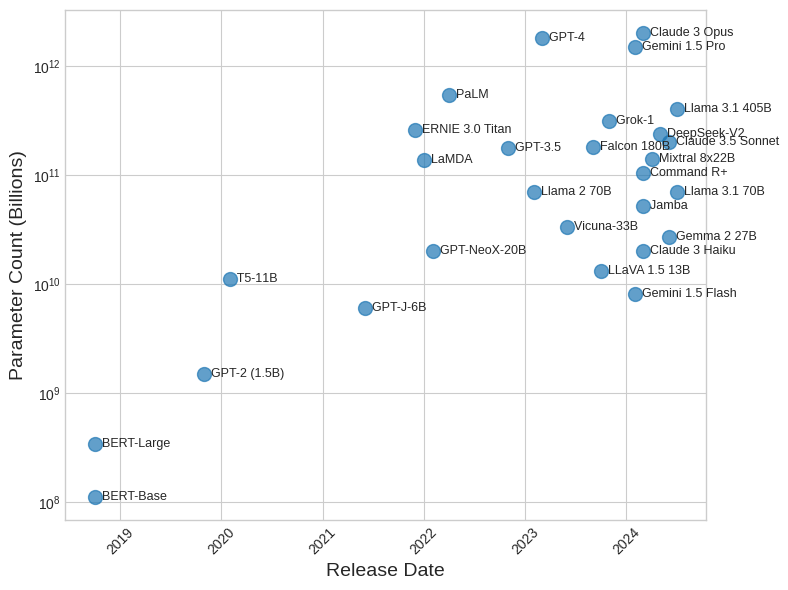
\includegraphics[width=0.8\textwidth]{images/llm_evolution.png}
            \caption{The evolution of LLMs.}
            \label{fig:llm_evolution}
        \end{figure}
        
        As highlighted by \citet{Singh2023}, the integration of LLM-based solutions, such as conversational chatbots, offers an approach to optimizing operations across various business segments, including drilling, completion, and production.
        \citet{Singh2023} uses LLMs models to extract, analyze, and interpret datasets, enabling generation of insights and recommendations. 

        Despite its widespread impact, language models are not without its limitations. 
        In many industry-specific applications, the critical information required is often proprietary, not shared with third parties, and thus absent from the training data of these LLMs \citep{Mosser2024}. 
        This gap means that GPT models might not have access to the most up-to-date or sensitive information needed for certain tasks. 
        Moreover, due to their probabilistic nature, LLMs can experience hallucinations, producing confident yet incorrect or nonsensical responses based on user input \citep{OpenAI2023}. 


    \section{Retrieval-Augmented Generation (RAG)}

        A RAG consists of two main components: a retriever and a generator, as illustrated in Figure~\ref{fig:rag_diagram}. The retriever is responsible for finding relevant information from a knowledge base, and the generator uses that information to create a human-like response. This approach has revolutionized natural language processing (NLP), allowing users to interact with databases using plain language rather than needing to know how to write complex SQL queries.

        \begin{figure}[h!]
            \centering
            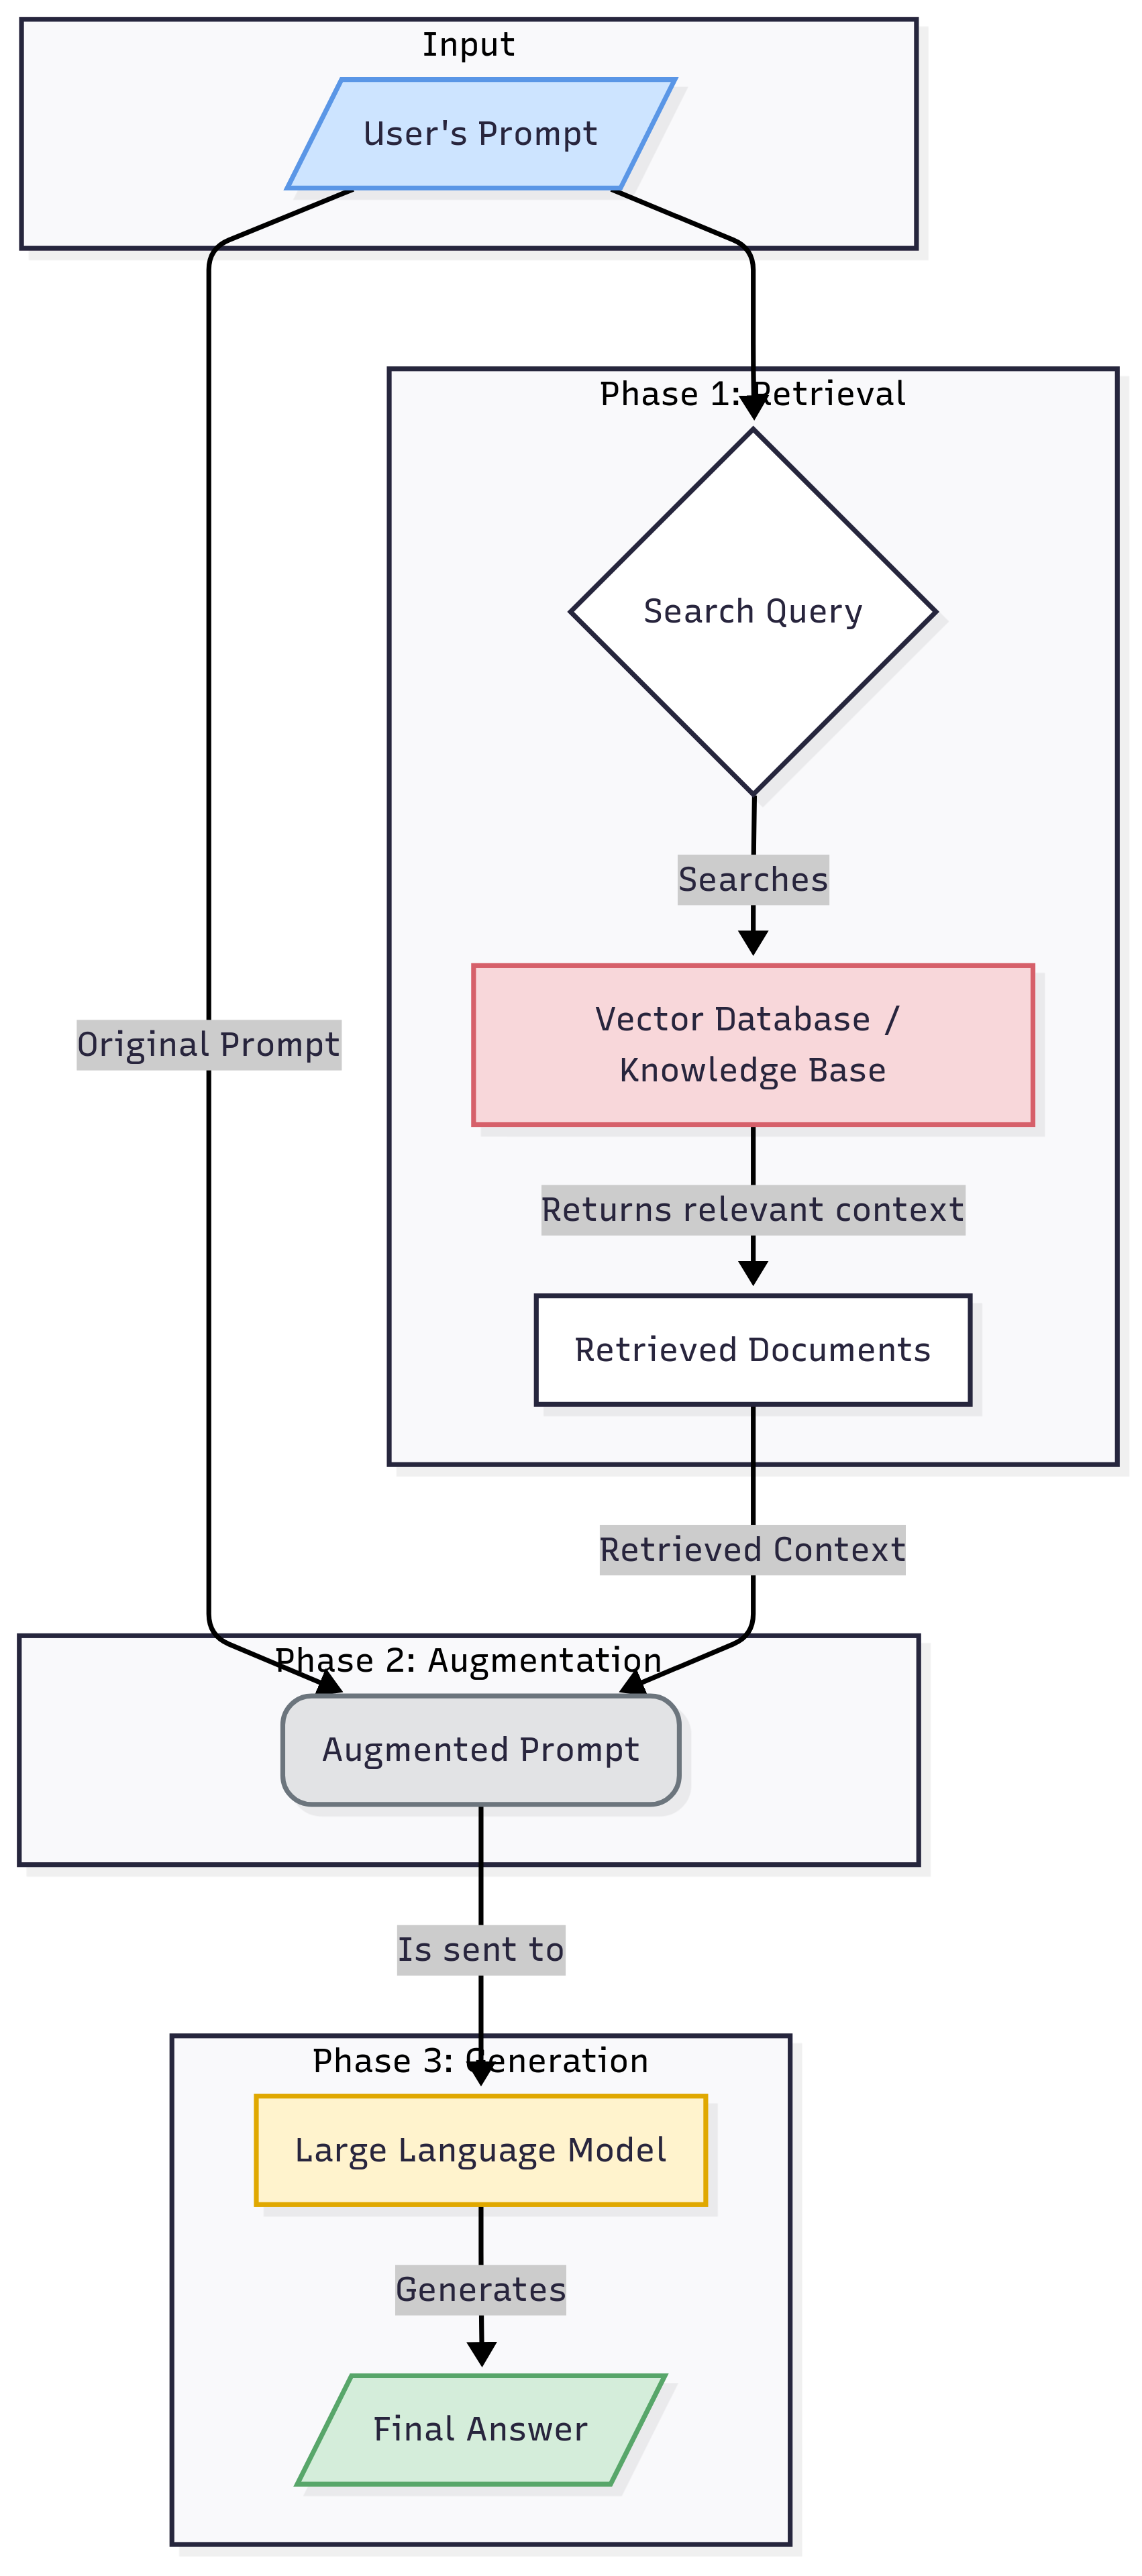
\includegraphics[width=0.4\textwidth]{images/rag_diagram_vertical.png}
            \caption{A diagram illustrating the RAG process.}
            \label{fig:rag_diagram}
        \end{figure}         
        
        The arrival of advanced language models like GPT-3 and GPT-4 \citep{OpenAImodels} has marked a significant leap in Text-to-SQL applications \citep{Singh2023}, demonstrating remarkable capabilities in handling these tasks. 
        This can be attributed to their extensive training on diverse datasets \citep{Deng2021}, which include not only large amounts of text but also structured data like tables and code, enabling the model to understand the intricate relationships between language and data structures. 
        The study by \citep{Deng2023} introduces a pre-training framework for text to SQL translation, emphasizing the alignment between text and tables in Text-to-SQL tasks.



    \section{Intelligent Agents}         
        % \xexeo{Agentes existem antes das LLMs, logo essa seção deve vir antes, inclusive já transformei em seção}
        % \vitor{feito}
        According to \citet{Russell2020}, an agent is something that performs actions. When it comes to computerized agents (in our case, AI-based), these agents are expected to do more: operate autonomously, perceive the environment, persist over time, adapt to changes, create, and strive to achieve goals.
        The agent program implements the agent function.
        There is a variety of basic agent program designs that vary in efficiency, compactness, and flexibility. The appropriate design of the agent program depends on the nature of the environment. In this work, a goal-based agent design was implemented, which acts to achieve defined goals \citep{Russell2020}.
        Other possible types include simple reflex agents, which directly respond to perceptions, while model-based reflex agents maintain an internal state to track aspects of the world that are not evident in the current perception. Finally, there are utility-based agents, which try to maximize their expected "happiness" \citep{Russell2020}.

    \section{LLM applications}

    % \todo[inline]{Precisa de um texto aqui}

        LLM applications have witnessed a dramatic surge in development and adoption, reshaping the landscape of AI. This growth is fueled by continuous advancements in model architectures, training techniques, and the availability of vast datasets. The proliferation of LLMs has led to a diverse array of applications that leverage their remarkable ability to understand, generate, and process human language.

        The expansion of the LLM application ecosystem is evident in the significant market growth projections. For instance, one report projects the global LLM market to grow from \$5.62 billion in 2024 to \$35.43 billion by 2030, with a compound annual growth rate (CAGR) of 36.9\% \citep{GrandViewResearch2025}. This rapid expansion is indicative of the immense value and potential that organizations across industries see in these technologies. The applications themselves are becoming increasingly sophisticated, evolving from simple text generation to complex, multimodal systems capable of processing and integrating text, images, and other data formats \citep{Kaddour2023}.
        
        The spectrum of LLM-based applications is broad and continually expanding. Early applications focused on tasks such as text summarization, translation, and sentiment analysis. However, the current generation of LLMs powers a much wider range of sophisticated tools. These can be broadly categorized into several key areas. Conversational AI, in the form of advanced chatbots and virtual assistants, represents a significant segment of the market, enhancing customer service and user engagement \citep{GrandViewResearch2025}. Content creation is another major application area, where LLMs are employed to generate a variety of materials, from marketing copy and social media posts to technical documentation and even creative writing \citep{V7Labs2025}.
        
        
        Furthermore, LLMs are being integrated into more specialized and high-stakes domains. In the legal field, they assist with tasks like contract analysis and legal research. The financial sector utilizes them for fraud detection and market analysis \citep{V7Labs2025}. In software development, LLM-powered tools for code generation and debugging are becoming increasingly prevalent, accelerating development cycles and improving programmer productivity. A key innovation driving the utility of these applications is the advent of techniques like Retrieval-Augmented Generation (RAG), which allows LLMs to retrieve and incorporate information from external knowledge bases, thereby improving the accuracy and relevance of their outputs \citep{KeywordsAI2025}. The ongoing development of multimodal LLMs is further pushing the boundaries of what is possible, enabling applications that can understand and reason about the world in a more holistic manner \citep{Kaddour2023}.
        
        \subsection{Retrieval-Augmented Generation (RAG)} 

            Retrieval-Augmented Generation (RAG) technique combines LLMs with information retrieval to generate accurate and up-to-date responses, as introduced by \citet{Lewis2020}. \xexeo{Aqui merece um desenho ilustrativo, até para quebrar tanto texto}
            It employs a search in a database to find relevant information, overcoming the inherent limitations of LLMs that rely solely on the prior knowledge embedded in the language model during the training phase. 
            With the ongoing evolution of information retrieval, which has moved from term-based methods to more semantic approaches leveraging deep learning and large datasets to tackle more complex challenges.
            
            As elucidated by \citet{Lewis2020}, RAG unites the strengths of pre-trained parametric and non-parametric memory, using a dense vector index and a semantic retriever. 
            As demonstrated by \citet{Li2022} in their analysis, RAG is surpassing traditional generative models in terms of performance across a variety of tasks. The study provides a detailed survey on this topic, emphasizing the fundamental concepts and its applicability in specific contexts.

            New tools have been developed to facilitate the implementation of RAG solutions. \citet{Liu2023} present a toolkit that integrates augmented retrieval techniques into LLMs, including modules for query rewriting, document retrieval, passage extraction, response generation, and fact-checking, enabling the creation of more factual and specific responses. The recent study by \citet{Zhao2023} extends this horizon by examining the incorporation of multimodal knowledge into generative models, exploring the integration of diverse external sources such as images, code, tables, graphs, and audio, to enhance the grounding context and improve usability. It also explores potential future trajectories in this emerging field, marking a relevant contribution to the evolving narrative of RAG and its applications.

            
        \subsection{Multi-Agent Setup} 

        \xexeo{Isso aqui seria uma seção de multi agentes dentro da LLM, mas você precisa escrever pelo menos um parágrafo de multi agentes gerais na seção agentes}      

            As demonstrated by \citet{xi2023rise}, the pursuit of Artificial General Intelligence (AGI) has significantly benefited from the development of LLM-based agents, capable of sensing, decision-making, and acting across diverse scenarios.  
            His study outline a foundational framework for such agents, consisting of brain, perception, and action components, which can be customized for various applications including single-agent scenarios, multi-agent systems, and human-agent collaboration . 
            The comprehensive survey underscores the crucial role of LLMs in moving towards AGI, suggesting a promising horizon for operational efficiency and decision-making processes in complex organizational settings \citep{xi2023rise}.

            \citet{Li2024} demonstrated that, through a sampling and voting method, the performance of LLMs scales with the number of instantiated agents.
            Another open-source framework is AutoGen \citep{Wu2023}, that enables the creation of LLM multi-agent applications, allowing for customization across various modes including. It supports diverse applications in fields such as mathematics, coding, and operations research, demonstrating its effectiveness through empirical studies \citep{Wu2023}.

        \section{LLM-as-judge}

        \xexeo{Òk, essa seção eu não gostei muito, apesar de não ter nenhum erro. Primeiro tem que fazer uma seção de avaliação com as medidas, onde devem estar todas as medidas que você usar na dissertação (não li ainda, estou indo na ordem). Aí então você pode falar disso, mas apenas se usou}

            The LLM-as-Judge paradigm represents a significant shift in the evaluation of NLP systems in general, using a language model as a scalable proxy for human evaluators (\citep{li2024llmsasjudgescomprehensivesurveyllmbased}). 
            This approach was developed to overcome the semantic shallowness of traditional metrics like BLEU or ROUGE and the logistical challenges of extensive human annotation (\citep{Zheng2023}). 
            By providing a "judge" LLM with a clear rubric and context, it can perform nuanced assessments of qualities like coherence, relevance, and factual accuracy (\citep{li2024llmsasjudgescomprehensivesurveyllmbased}).
            This method has proven effective for complex, open-ended tasks where simple string matching is insufficient, with models like GPT-4 demonstrating over 80\% agreement with human preferences in benchmarking studies \citep{Zheng2023}.

            For evaluating Retrieval-Augmented Generation (RAG) systems, the LLM-as-Judge framework can be adapted to produce structured, quantitative assessments. 
            In this application, the judge LLM is tasked with comparing the RAG-generated answer against a ground-truth dataset.
            By leveraging a meticulously crafted prompt that defines the classification criteria, the judge can systematically categorize each output into classes such as True Positive (TP) (factually consistent with the ground truth), False Positive (FP) (introduces unsupported information), True Negative (TN) (a correct refusal to answer), or False Negative (FN) (missing relevant information). This structured approach moves beyond subjective scoring towards a more objective, task-specific evaluation, similar to methodologies that use specialized judge models trained on fine-grained feedback for enhanced reliability (\citep{Kim2024}).

            The primary advantage of this methodology is its ability to translate qualitative, AI-driven judgments directly into a confusion matrix. By aggregating the classifications across an entire evaluation dataset, it becomes possible to calculate standard, interpretable metrics such as precision (Equation~\ref{eq:precision}), recall (Equation~\ref{eq:recall}), and F1-score (Equation~\ref{eq:f1-score}). This process establishes a robust and replicable pipeline for benchmarking the factual accuracy of a RAG system at scale. While it is important to acknowledge the potential for inherent biases in LLM judges (\citep{Gu2025}), studies show high correlation with human-expert evaluations (\citep{li2024llmsasjudgescomprehensivesurveyllmbased}), making it a powerful tool for iterative development and system comparison.

            \begin{equation}
                \text{Precision} = \frac{\text{TP}}{\text{TP} + \text{FP}}
                \label{eq:precision}
            \end{equation}

            \begin{equation}
                \text{Recall} = \frac{\text{TP}}{\text{TP} + \text{FN}}
                \label{eq:recall}
            \end{equation}

            \begin{equation}
                \text{F1-score} = 2 \times \frac{\text{Precision} \times \text{Recall}}{\text{Precision} + \text{Recall}}
                \label{eq:f1-score}
            \end{equation}

\todo[inline]{Como você criou um dataset de teste para uma tarefa, seria bom falar disso. Mas essa é uma coisa adicional a outras mudanças que pedi, seria bom, mas se não der tempo, não deu.}

\todo[inline]{Você usou no prmeiro experimento outras métricas, tem que descreve-las aqui: Truthfulness, Performance, LLMCost}
